\documentclass[english,notitlepage,reprint,nofootinbib]{revtex4-1}  

\usepackage[utf8]{inputenc}


\usepackage{physics,amssymb}  % mathematical symbols (physics imports amsmath)
\include{amsmath}
\usepackage{graphicx}         % include graphics such as plots
\graphicspath{{../plots/}}
\usepackage{xcolor}           % set colors
\usepackage{hyperref}         % automagic cross-referencing
\usepackage{listings}         % display code
\usepackage{subfigure}        % imports a lot of cool and useful figure commands
% \usepackage{float}
%\usepackage[section]{placeins}
\usepackage{algorithm}
\usepackage[noend]{algpseudocode}
\usepackage{subfigure}
\usepackage{enumitem} 
\usepackage{tikz}
\usetikzlibrary{quantikz}
\hypersetup{
    colorlinks,
    linkcolor={red!50!black},
    citecolor={blue!50!black},
    urlcolor={blue!80!black}}

\setlist[itemize]{noitemsep}
\setlist[enumerate]{noitemsep}
\setlist[itemize]{nolistsep}
\setlist[enumerate]{nolistsep}

% ===========================================


\begin{document}

\title{FYS-STK4155 Projec 3}  % self-explanatory
\author{Keran Chen and Torstein Bjelland} % self-explanatory
\date{\today}                             % self-explanatory
\noaffiliation                            % ignore this, but keep it.

%This is how we create an abstract section.
\begin{abstract}
	The purpose of this project was to analyse the well known red wine quality data originally proposed by Cortez et al. \cite{CORTEZ2009547} using machine learning methods including linear models: Ordinary Least Square (OLS), Ridge and Lasso regression, Feed Forward Neural Network (FFNN) decision trees and random forest. We found that decision trees using random forest as ensemble method produced the best predictions with accuracy of $ 65\% $ to $ 75\% $ regardless whether the problem is treted as a regression or a classification problem. This accuracy is higher than the $ 57.7\% $ to $ 67.5\% $ by the authors of the original paper using Support Vector Mechines with tolerance of $ 0.5 $ . We found also that the maximum depth for the decision trees that produced the best results is $ 15 $ using accuracy scores and not mean square error. The typical problem of overfitting was not seen on decision trees with or without random forest ensemble and we did not rule out the possibility that it is due to the data itself had very low variance. 
\end{abstract}

\maketitle

\begingroup\small\noindent\raggedright\textbf{Source code}\\
The source code, data, and/or other artifacts have been made available at \url{https://github.com/KlogeBukser/mlproj3}.
\endgroup

% ===========================================
\section{Introduction}
The ultimate goal for machine learning is to analyse data, if only there were one almighty algorithm that perfectly fits all the curves and predicts the result. In reality, however, the best machine learning algorithms is often subject to the specific dataset. It thus become an essential and interesting topic to identify the best method for a particular dataset.\\
This project surrounds the \textit{Wine Quality Data} \cite{CORTEZ2009547} that is both available from Kaggel \cite{learning_2017} and UCL Machine Learning Repository~\cite{uci2009}, with the goal being to identify the quality of the wine using its physiochemical properties. By doing so we compare the performance of different machine learning methods and identify the best parameters (specific to the data). The methods employed here are Linear Regression, Feed Forward Neural Network (FFNN) and Decision Trees, all from the \textit{scikit-learn} library. The theory of the used machine learning methods are first presented, with those appeared in project 1 or 2 omitted. In Section~\ref{sec:results}, a visual representation of the dataset is presented, followed by the data analysis results from machine learning, then a discussion of the results in Section~\ref{sec:discussion}, before concluding the finding in Section~\ref{sec:conclusion}.

%

% ===========================================
\section{Methods}\label{sec:methods}
%
As mentioned in the introduction, methods used in project 1 and 2 are not repeatedly discussed. 

\subsection{Decision Tree}
A tree contains a root node, the interior nodes, and the final leaf nodes, while the connections between nodes are called branches. First, a decision tree tries to split its values into, mostly 2, but sometimes more, subbranches using the CART algorithm in our case. Then the above mentioned step is repeated at each sub-node and the tree grows recursively until the given depth or until there is no more impurity in the subset. In general, without regularisation, decision trees are prone to overfitting and have high variance.

\subsection{The CART algorithm}\label{sub:cart}
CART stands for Classification And Regression Tree. In the case of classification, the Gini factor $ G $ was use determine the impurity. The cost function we are trying to minimise is:
\[ C(k,t_k) = \frac{m_{\mathrm{left}}}{m}G_{\mathrm{left}}+ \frac{m_{\mathrm{right}}}{m}G_{\mathrm{right}} \] 
where $ k $ is a single feature and , $ t_k $ is a threshold, and $G_{\mathrm{left/right}}$ measures the impurity of the left/right subset  and $m_{\mathrm{left/right}}$ is the number of instances in the left/right subset.

For regression, we try to minimise the Mean Square Error (MSE), the cost function is then:
\[C(k,t_k) = \frac{m_{\mathrm{left}}}{m}\mathrm{MSE}_{\mathrm{left}}+ \frac{m_{\mathrm{right}}}{m}\mathrm{MSE}_{\mathrm{right}}. \]

note that MSE for a specific node is defined as 
\[ \mathrm{MSE}_{\mathrm{node}}=\frac{1}{m_\mathrm{node}}\sum_{i\in \mathrm{node}}(\overline{y}_{\mathrm{node}}-y_i)^2, \] 
with 
\[ \overline{y}_{\mathrm{node}}=\frac{1}{m_\mathrm{node}}\sum_{i\in \mathrm{node}}y_i. \] \cite{hjorth-jensen}

\subsection{Random Forest}
Random forest is an extension from bagging, which is an ensemble method that splits the training data into smaller subsets and build decision tree on each subset. It in general reduces variance. \\ Random forest utilises both bagging and feature randomness to create an uncorrelated forest of decision trees. For a regression task, the individual decision trees will be averaged, and for a classification task, a majority vote—i.e. the most frequent categorical variable—will yield the predicted class. \cite{ibm}. 
At each split, we choose $ m $ predictors from $ p $ predictors, typically with
\[ m\approx \sqrt{p}. \] 

We will grow of forest of say $B$ trees. 
\begin{enumerate}
	\item  For $b=1/B$: 
		\begin{itemize}
			\item Draw a bootstrap sample from the training data organized in our $\boldsymbol{X}$ matrix.
			\item We grow then a random forest tree $T_b$ based on the bootstrapped data by repeating the steps outlined till we reach the maximum node size is reached. 
		\end{itemize}

	\item Select $m \le p$ variables at random from the $p$ features
	\item pick the best split point among the $m$ features using for example the CART algorithm and create a new node
	\item split the node into daughter nodes
	\item Output then the ensemble of trees $\{T_b\}_1^{B}$ and make predictions for either a regression type of problem or a classification type of problem. 
\end{enumerate} \cite{hjorth-jensen}
%

% ===========================================
\section{Results}\label{sec:results}
%
The data was split into training and testing data using 8:2 ratio. If the result is plotted against multiple runs, the same training and testing data is used unless otherwise specified. \\
In some results from regression models, the predicted values are rounded to the nearest integer to discretise them. Since \textbf{Quality} (i.e. what's being predicted) is a discrete variable, we can calculate the accuracy scores and graph a confusion matrix as we would a classification problem. 
\subsection{Dataset}

\begin{figure}[H]
	\centering
	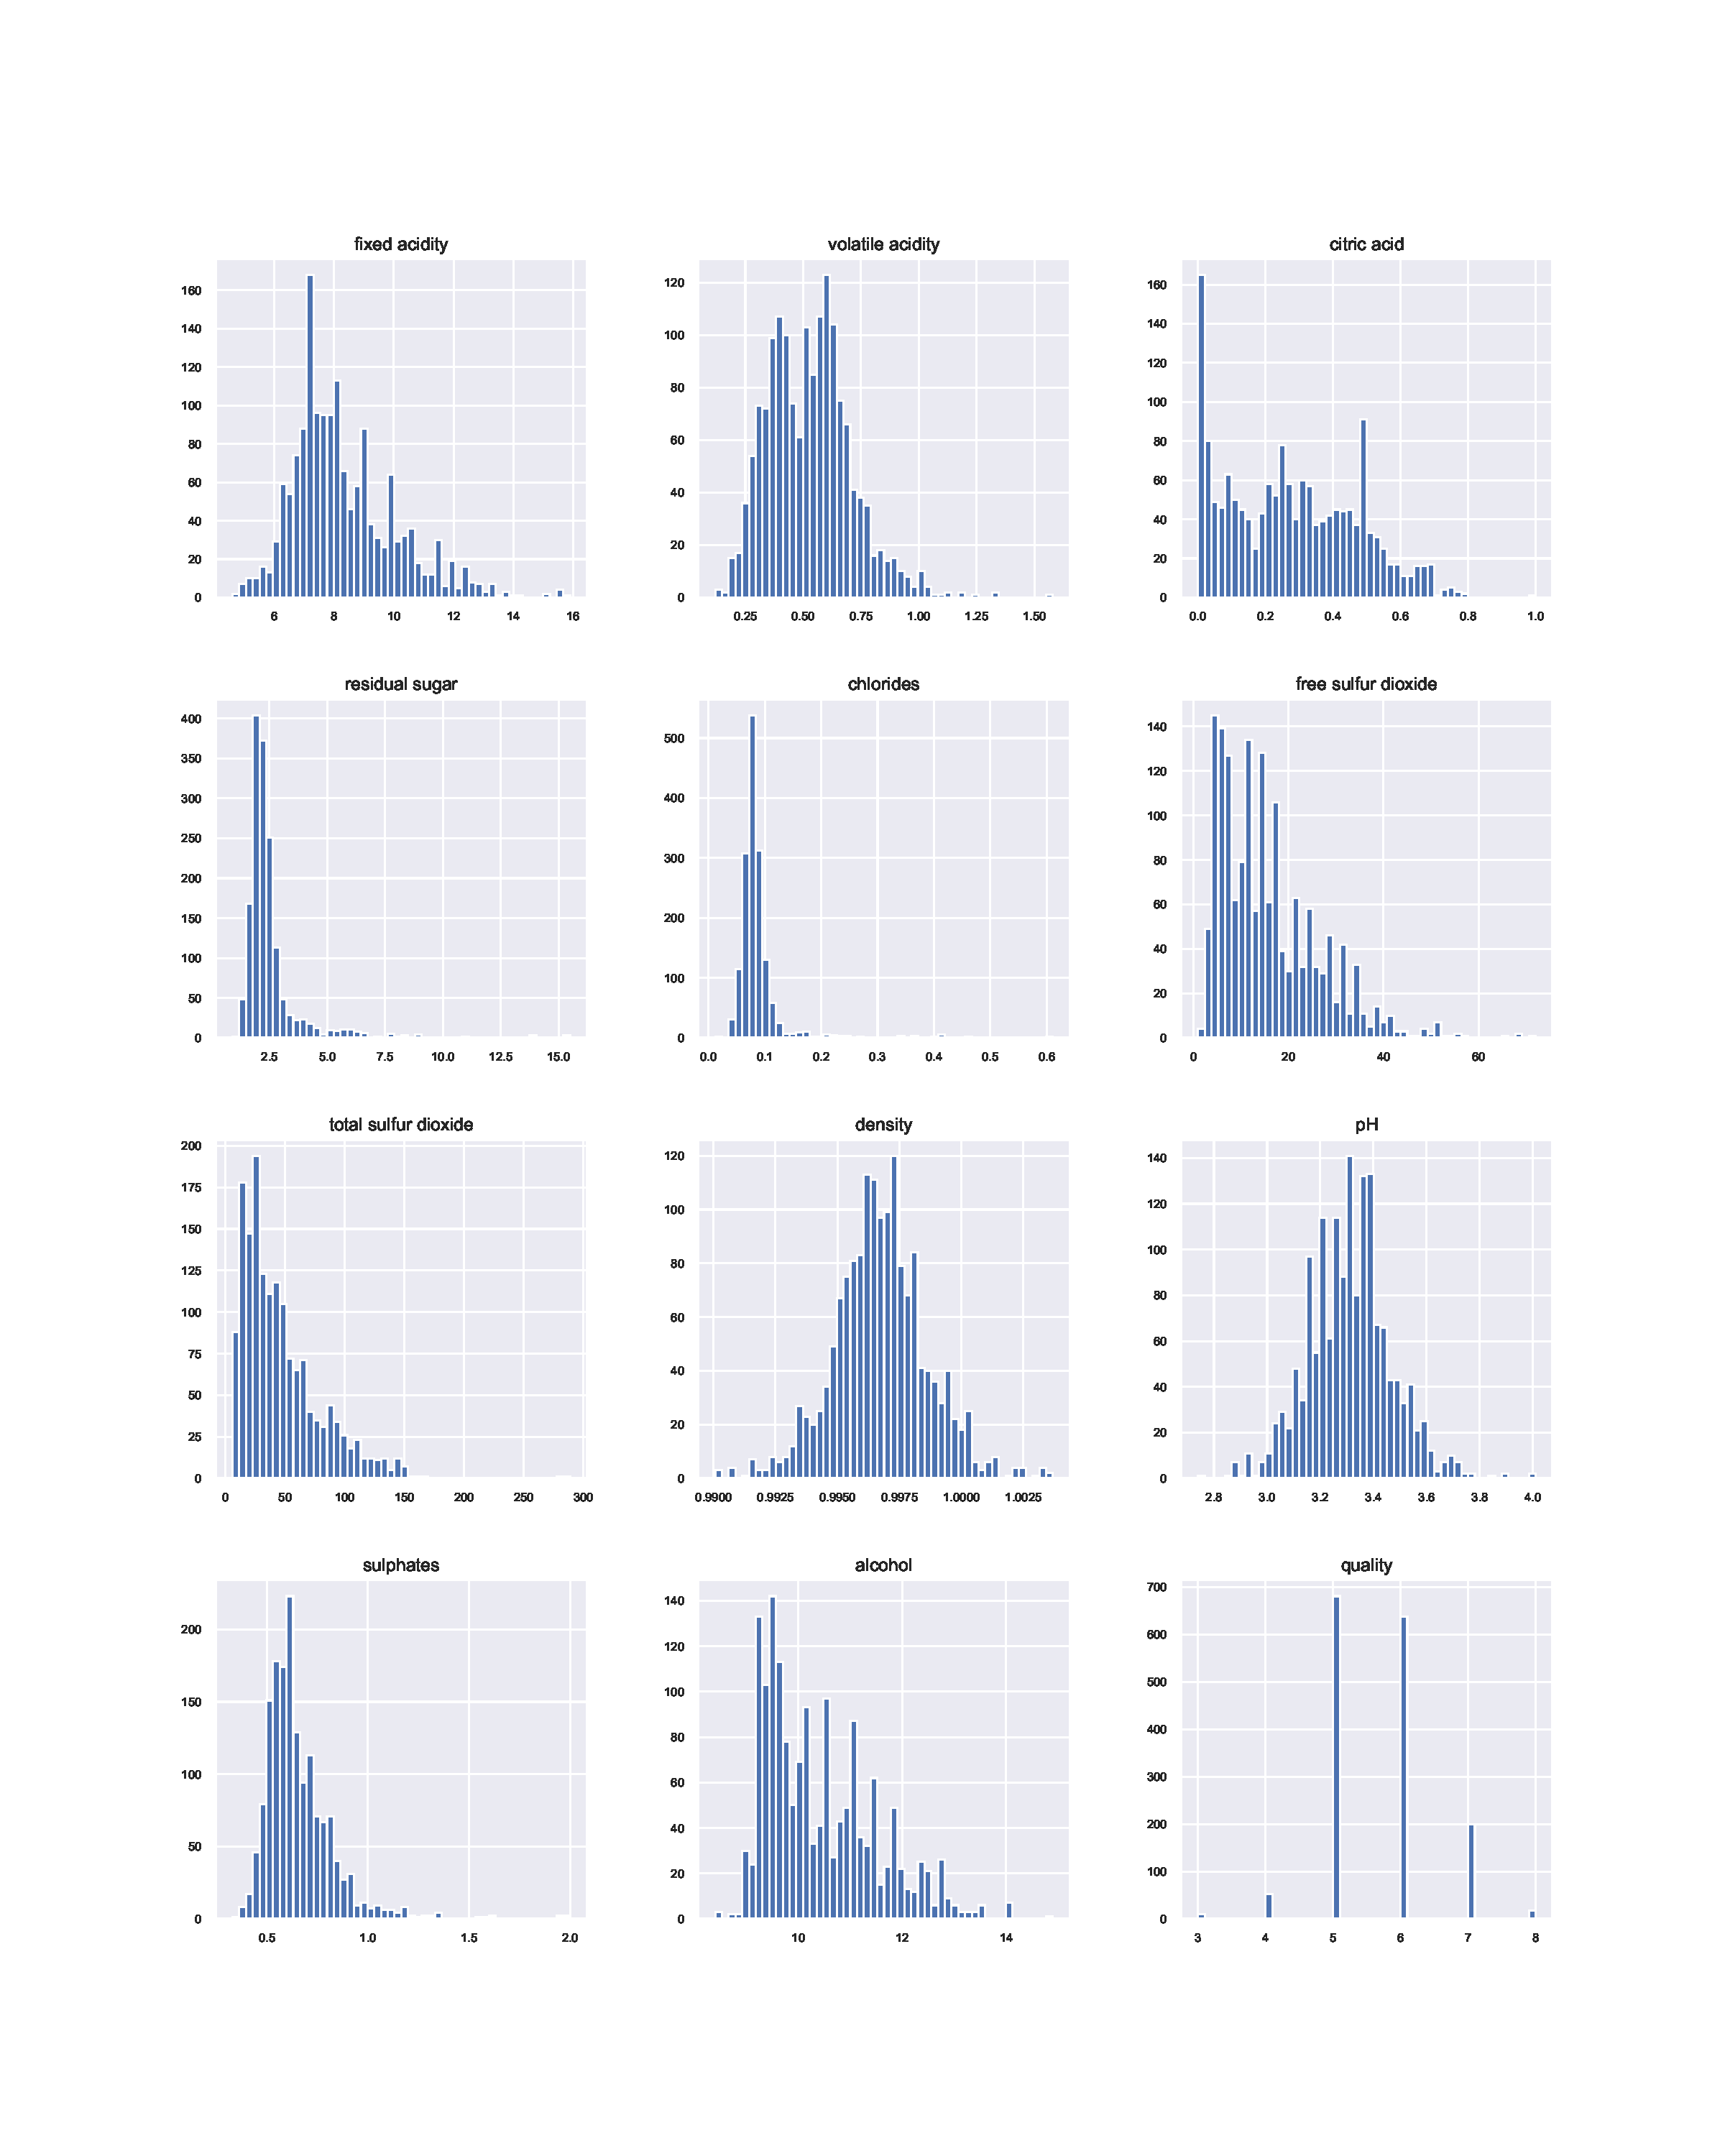
\includegraphics[width=\linewidth]{data-visualisation.pdf}
	\caption{Histograms of Features of the dataset.}
	\label{fig:datavis}
\end{figure}


\begin{figure}[H]
	\centering
	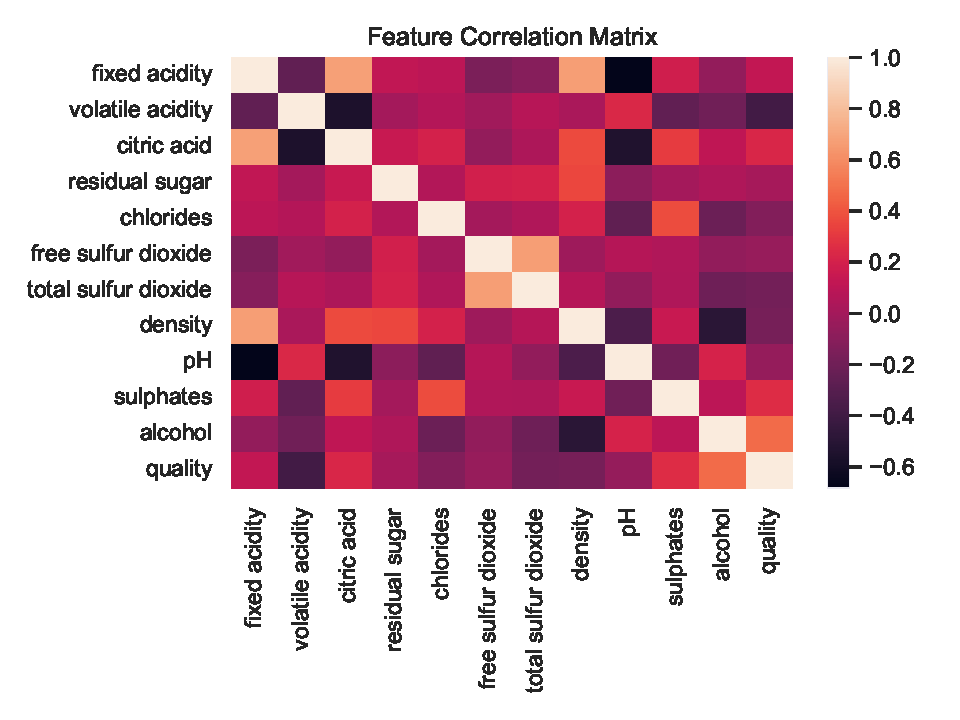
\includegraphics[width=\linewidth]{feature-corr.pdf}
	\caption{Correlation between features of the dataset.}
	\label{fig:featcorr}
\end{figure}

\subsection{Linear Regression Results}

\begin{figure}[H]
	\centering
	\includegraphics[width=\linewidth]{lin_rgn-hyperparams.pdf}
	\caption{L1 (Lasso) and L2 (Ridge) hyperparameters tuning results, the hyperparameters $ \lambda \in [10^{-4}, 1]$ for 1000 logarithmically spaced points.}
	\label{fig:lintune}
\end{figure}

\begin{figure}[H]
	\centering
	\includegraphics[width=\linewidth]{lin_rgn-ols-cm.pdf}
	\caption{Confusion matrix of OLS predictions.}
	\label{fig:olscm}
\end{figure}


\subsection{Neural Network}
\begin{figure}[H]
	\centering
	\includegraphics[width=\linewidth]{../plots/nn-methods-cm(500 iter).pdf}
	\caption{Confusion matrix for different learning rate update methods and activation functions taking average of 500 runs.}
	\label{fig:nn-method}
\end{figure}

\begin{figure}[H]
	\centering
	\includegraphics[width=\linewidth]{nn-hidden-cm.pdf}
	\caption{Heatmap for different number of layers and number of hidden nodes for a fully connected neural network, average over 10 runs each.}
	\label{fig:nn-hidden}
\end{figure}

\begin{figure}[H]
	\centering
	\includegraphics[width=\linewidth]{nn-rgn-cm.pdf}
	\caption{FFNN regression result for 1 layer with 100 nodes, using Sigmoid as activation functions and constant learning rate updates.}
	\label{fig:nn-rgn-cm}
\end{figure}

\subsection{Decision Trees}

\begin{figure}[H]
	\centering
	\includegraphics[width=\linewidth]{tree-rgn-scoresVSdepth[1,20].pdf}
	\caption{Tuning results for decision tree regressor. Mean scores for 1000 runs are plotted against maximum depth $ \in [1,20] $  with steps of $ 2 $  of the tree. }
	\label{fig:tree-rgn-tune}
\end{figure}

\begin{figure}[H]
	\centering
	\includegraphics[width=\linewidth]{../plots/tree-clf-scoresVSdepth[1,45].pdf}
	\caption{Tuning results for decision tree classifier. Mean scores for 1000 runs are plotted against maximum depth $ \in [1,41] $ with steps of $ 5 $  of the tree.}
	\label{fig:tree-clf-tune}
\end{figure}

\begin{figure}[H]
	\centering
	\includegraphics[width=\linewidth]{../plots/tree-forest-rgncm.pdf}
	\caption{Random forest confusion matrix result for regression, with max depth 15.}
	\label{fig:forest-rgncm}
\end{figure}

\begin{figure}[H]
	\centering
	\includegraphics[width=\linewidth]{tree-forest-clfcm.pdf}
	\caption{Random forest confusion matrix result for classification, with max depth 15.}
	\label{fig:forest-clfcm}
\end{figure}

\begin{figure}[H]
	\centering
	\includegraphics[width=\linewidth]{tree-forest-scores15.pdf}
	\caption{Random forest regressor and classifier result compared. Accuracy plotted against 100 runs, with max depth 15. }
	\label{fig:forest-compared}
\end{figure}

\begin{figure}[H]
	\centering
	\includegraphics[width=\linewidth]{final-cmp.pdf}
	\caption{Comparison of all methods: OLS, Ridge, Lasso, FFNN, Random Forest Regressor, Random Forest Classification. Accuracy scores is plotted against index of runs, each run resamples training and testing data.}
	\label{fig:final-cmp}
\end{figure}


% ===========================================
\section{Discussion}\label{sec:discussion}
%

\subsection{the data}
It is a good practice to first look at the dataset before attempting to solve any problem. The histogram in Figure~\ref{fig:datavis} indicates that a lot of the features are normally distributed, rather than uniformly distributed (i.e. the data is not balanced). This might cause our machine learning algorithms to favour the prediction of an "average wine" to a "great wine" or a "horrible wine". The correlation matrix in Figure~\ref{fig:featcorr} shows no surprising correlation, except the obvious ones such as "citric acid" and "total acidity" or "free sulfur dioxide" and "total sulfur dioxide". Thus all the features are included in training.


Considering the nature of the problem, this is clearly a regression problem. Even though the values are discrete, there is a clear ordering in term of the quality, as in, a `7` is better than a `6` which is in turn better than a `5`. This is indeed what we started off doing. However, because of the way the dataset is presented -- the value we are trying to predict, \textit{Quality}, is a discrete variable. It is tempting to treat this is a classification problem. We employed both a classifier and a regressor when using Decision Tree found some interesting results.


\subsection{Parameters}
For linear regression methods, it is again the $ L_1 $ and $ L_2 $ regularisation parameters that need to be tuned. According to Figure~\ref{fig:lintune} Ordinary Least Square performed the best. This does not come as a surprise the regularisation parameters help preventing overfitting and reduce influences from outlier but our data does not contain many outliers, but has rather a low variance.  \\
For FFNN, which learning rate update method we use seemed to have tiny influence on the performance of the model, with constant update being the best. The best activation functions are the $ \tanh $and the \textit{logistic} (Sigmoid) function. From Figure~\ref{fig:nn-hidden}, the best size of the FFNN is $ 1 $ layer with $ 100 $ nodes in the layer. This also happened to be the default values. It also seems like that in general models with fewer layers performed better. \\
Figure~\ref{fig:tree-rgn-tune} and Figure~\ref{fig:tree-clf-tune} was created in order to determine what is the best maximum depth for a decision tree. All three scores were included in order to do compare between the two. The best max depth which minimises MSE is however not the parameter that maximises accuracy. Ultimately I've chosen accuracy over MSE. We discovered that the accuracy initially increased rapidly with max depth, then rounded of around $ 15 $ and decided max depth of $ 15 $ is the best depth to use. This depth is also used for all the random forest result produced.


\subsection{Regression or Classification?}
The random forest results produced using max depth $ =15 $ (Figure~\ref{fig:forest-rgncm} and
Figure~\ref{fig:forest-clfcm}) are very similar and they have similar accuracy as seen on Figure~\ref{fig:forest-clfcm}. Counter-intuitively, the classifier perform as well as the regressor. This perhaps indicates at the heart of decision trees (and indeed neural networks and many others), there is really not that big of a different between a regression and classification problem. In the case of a decision tree, both uses the CART algorithm mentioned in Section~\ref{sub:cart}. The only difference is whether square loss or Gini index was used as the loss function. 


\subsection{Comparisons}
The best performing linear model is OLS, which 
Figure~\ref{fig:final-cmp} shows that random forests perform much better than FFNN which performs similar the linear models. The former consistently produced results with accuracies ranging from $ 65\% $ to $ 75\% $, while the latter produced results with accuracies ranging from $ 53\% $ to $ 68\% $. Interestingly, the decision trees with max depth of $ 15 $ doesn't seem to be overfitting, this might again be caused by the dataset being very centered (disproportional number of 5's and 6's ).

\subsection{Link to Other Researches}
The researchers who published paper on the dataset originally, (Cortez et al.) used Mean Absolute Deviation, i.e. Mean absolute error, (MAE) instead of Mean Square Error (MSE), which is perhaps a better metric than accuracy which we have used here since it takes into account how far away the predictions are when it's inaccurate. As mentioned earlier, the dataset is unbalanced and would not perform well in identifying the outliers naturally. Looking at Figure~\ref{fig:nn-rgn-cm} and indeed Figure~\ref{fig:forest-rgncm} and \ref{fig:forest-clfcm}, we see that all the results are in the center of the heatmap, indicating that our model is not ``very off`` when the result isn't correct. This information is missing from Accuracy but indeed captured and quantified by MAE. \\

They have also used sensitive analysis for NN in which the every iteration removes the least sensitive neurons, which outperformed back propagation and genetic algorithms. \\

Cortez et al. concluded that Support Vector Machine is the best method to analyse this dataset, with accuracy between $57.7\%$ to $67.5\%$ for a tolerance of $ 0.5 $ (only the correct class) and a whopping result between $ 81.9\% $ to $100\%$ with tolerance of $ 1.0 $. \cite{CORTEZ2009547}
% ===========================================
\section{Conclusion}\label{sec:conclusion}
After exploring different parameters and methods. We found that, specific to this dataset, a random forest approach performs the best with maximum of depth of $ 15 $.It has accuracy score between $ 65\% $ to $ 75\% $. This performance is better than best result of $ 57.7\% $ to $ 67.5\% $ produced by Cortez et al. using Support Vector Machine with tolerance $ =0.5 $. \cite{CORTEZ2009547} FFNN has similar performance to linear regression models, but takes much longer to run. They produced accuracies between $57.7\%$ to $67.5\%$. \\
The performance of all methods are clearly correlated to how the data is split. We have also discovered that we could get similar results by treating the wine quality problem as a classification problem, however counter intuitive it is. The models have a common problem that is they favour predicting average values than more extreme values. This is inherent from the unbalanced nature of the dataset. This, however, might be the reason why the decision trees methods are overfitting the data, as they are very centered with few outliers.


\subsection{Further Evaluation}\label{sec:evaluation}
Independent analysis using Support Vector Machines could be the next step. It is not included in this project as we didn't read the paper by Cortez et al. \cite{CORTEZ2009547} until we finished most of the analysis. Outlier detection algorithms could also be explored on this dataset due to its unbalance. One could also treat this at a classification problem by simply using quality $ \ge 7 $ to be a `good wine` and otherwise a `bad wine` \cite{learning_2017}. Finally one could test different cost functions (MSE, MAE, accuracy) and see which one better evaluates the models. Quantitative time performance of different methods can also be interesting topic for further exploration.

\section{Appendix: Non-essential plots}
\begin{figure}[ht]
	\centering
	\includegraphics[width=\linewidth]{../plots/lin_rgn-ridge-cm.pdf}
	\includegraphics[width=\linewidth]{../plots/lin_rgn-lasso-cm.pdf}
	\caption{Confusion matrices for ridge and lasso regression results.}
	\label{fig:ridge-lasso-cm}
\end{figure}


\onecolumngrid

%\bibliographystyle{apalike}
\bibliography{ref}


\end{document}
